%试卷模板
\documentclass[a3paper,twocolumn,2twoside,landscape,12pt,UTF8]{ctexart}
\setlength{\columnsep}{36pt}
\usepackage{latexexercise0}
%教案模板
% \documentclass[12pt,UTF8]{ctexart}
% \usepackage{latexexercise}
\usepackage{QingDa}
\usepackage{multirow}
%\usepackage{subfig}
\usepackage[hypcap=true,labelsep=period,font=small]{caption}% 图的标题设置Fig.
\usepackage[hypcap=true]{subcaption}%用于画子图 可以适配hyperref包
\usepackage{float}

\pgfplotsset{width=6cm,compat=1.15}
\newcommand\putfig[2]{\begin{tabular}[t]{@{}l@{}}#1\\#2\end{tabular}}
\begin{document}

% \Grade{高一}
\Name{1v2}\FirstTime{20181028}\CurrentTime{20181117}
% \Name{郭文镔}\FirstTime{20181111}\CurrentTime{20181117}
% \Name{马灿威}\FirstTime{20181111}\CurrentTime{20181111}
\Topic{任意角、弧度制与三角函数}
\Teach{任意角的三角函数}
\makefront
\vspace{-1.5em}
\startexercise

\hspace{-2.5em}
{\hei 本章节学习内容}\par
1. 建立一般三角函数的概念,并研究函数性质,包括周期性、奇偶性、单调性与最值;\par
2. 探索和研究三角函数之间的一些恒等关系;\par
3. 利用三角函数构建数学模型,解决实际问题。\par

\section{任意角与弧度制}
\subsection{预备知识}
1. 角与角度的概念;集合的表示;不等式的基本性质;集合的运算;直线的倾斜角;\par
2. 角度制;圆心角的性质;比例、分数的性质;圆的周长与面积;弦长的计算;锐角三角函数;二次函数最值/基本不等式.\par
\subsection{问题导学}
{\heiti 【思考1】}:角的概念是怎么产生的?我们生活中在什么时候用到过角的概念?\par
\vspace{6em}
{\heiti 【思考2】}:我们学过的角的定义是?能说出为什么这样定义么?这样定义的角可以应用在哪里呢?\par
\vspace{10em}
{\heiti 【思考3】}:为什么要定义角度?我们学过的角度是如何定义的?角度如何运算?\par
\vspace{10em}

% \begin{exercise}{习题}
% \item
% 下列说法正确的是\xz
% \xx{终边相同的角一定相等}
% {钝角一定是第二象限角}
% {第一象限角一定不是负角}
% {小于90\textdegree 的角都是锐角}
% \begin{answer}B\end{answer}
%
% \end{exercise}
\section{任意角的三角函数}
\subsection{预备知识}
1. 锐角三角函数;函数定义域
2. 勾股定理;开方;代数式化简,完全平方公式;一元二次方程求解
\subsection{问题导学}
{\heiti 【思考1】}:锐角三角函数的定义是?为什么要定义三角函数呢?三角函数有哪些应用?\par
\vspace{12em}
{\heiti 【思考2】}:锐角三角函数之间有什么关系呢?\par
\vspace{12em}

% \section{课后作业}


\stoptexercise

% % sty文件使用 \RequirePackage{latexexercise0}
% 主文件使用 \documentclass[a3paper,twocolumn,2twoside,landscape,12pt,UTF8]{ctexart}
\hspace{3cm}\\
\vspace{0.5cm}
\centering{\heiti \xiaoer 福州八中2018-2019学年第一学期期中考试}\\
\vspace{0.5cm}
\centering{\heiti \erhao 高一数学\quad 必修一}\\
\vspace{0.4cm}
\centering{\wuhao 考试时间:120分钟\hspace{5em}试卷满分:150分}\\
\vspace{-1.6em}
\part{第I卷}
\vspace{-3em}
\startexercise
\begin{exercise}
\section{选择题(本大题共10小题,每小题5分,共50分.每题有且只有一个选项是正确的,请把答案填在答卷相应位置上)}
\item
设集合$A=\{x\in\mathbb{Q}|x>1\}$,则\xz
  \xx{$\varnothing\in A$}
  {$\sqrt2\notin A$}
  {$\sqrt2\in A$}
  {$\{\sqrt2\}\subseteq A$}
\begin{answer}
  B
\end{answer}
\item
下列函数中与函数$y=x(x\geq 0)$有相同图像的一个是\xz
  \xx{$\displaystyle y=\frac{x^2}x $}
  {$y=\sqrt{x^2}$}
  {$y=\sqrt[3]{x^3}$}
  {$y=(\displaystyle \sqrt x)^2 $}
\begin{answer}
  D
\end{answer}
\item
下列函数在区间$(0,+\infty) $上是增函数的是\xz
  \xx{$y=\ln(x+1)$}
  {$y=(x-1)^2$}
  {$y=x^{-2}$}
  {$y=3^{-x}$}
\begin{answer}
  A
\end{answer}
\item
设$f(x)=\begin{cases}
  x-2,x\geq10\\f[f(x+6)],x<10
\end{cases}$,则$f(9)$的值为\xz
  \xx{10}{11}{12}{13}
\begin{answer}
  B
\end{answer}
\item
若函数$f(x)=x^3+x^2-2x-2$的一个正数零点附近的函数用二分法计算,其参考数据如下:\\
\begin{center}
  \begin{tabular}{|c|c|c|}
    \hline
    $f(1)=-2$&$f(1.5)=0.625$&$f(1.25)=-0.984$\\
    \hline
    $f(1.375)=-0.260$&$f(1.4375)=0.162$&$f(1.40625)=-0.054$\\
    \hline
  \end{tabular}\\
\end{center}
那么方程$x^3+x^2-2x-2=0$的一个近似根(精确度$0.1$)是\xz
  \xx{1.2}
  {1.3}
  {1.4}
  {1.5}
\begin{answer}
  C
\end{answer}
\item
已知函数$f(x)$的值域为$[-2,3]$,则函数$f(x-2)$的值域为\xz
  \xx{$[-4,1]$}
  {$[0,5]$}
  {{$[-4,1]\cup[0,5]$}}
  {$[-2,3]$}
\begin{answer}
  A
\end{answer}
\item
三个数$0.8^9,9^{0.8},\log_{0.8}9$的大小关系为\xz
  \xx{$\log_{0.8}9<0.8^9<9^{0.8}$}
  {$0.8^9<9^{0.8}<\log_{0.8}9$}
  {$\log_{0.8}9<9^{0.8}<0.8^9$}
  {$0.8^9<\log_{0.8}9<9^{0.8}$}
\begin{answer}
  A
\end{answer}
\item
函数$f(x)=1+\log_2x$与$g(x)=2^{-(x-1)}$在同一直角坐标系下的图像大致是\xz
\begin{tikzpicture}
  \coordinate[label=below left:$O$] (O) at(0,0);
  \draw[->,>=latex](-0.8,0)--(3.6,0)node[below](x){$x$};
  \draw[->,>=latex](0,-1.5)--(0,3.2)node[left](y){$y$};
  \draw[domain=0.4:3]plot(\x,{log2(\x)});
  \draw[domain=-0.5:3]plot(\x,{pow(2,1-\x)});
  \draw[dashed](1,0.1)--(1,0)node[below](x1){$ 1 $};
  \draw[dashed](2,0.1)--(2,0)node[below](x2){$ 2 $};
  \draw[dashed](0.1,1)--(0,1)node[left](y1){$ 1 $};
  \draw[dashed](0.1,2)--(0,2)node[left](y2){$ 2 $};
  \coordinate[label=$\mathrm{A}$](a) at(1.5,-2);
  \begin{scope}[xshift=4.7 cm]
    \coordinate[label=below left:$O$] (O) at(0,0);
    \draw[->,>=latex](-0.8,0)--(3.6,0)node[below](x){$x$};
    \draw[->,>=latex](0,-1.5)--(0,3.2)node[left](y){$y$};
    \draw[domain=0.4:3]plot(\x,{0.1+log2(\x)});
    \draw[domain=-0.7:3]plot(\x,{pow(2,-\x)});
    \draw[dashed](1,0.1)--(1,0)node[below](x1){$ 1 $};
    \draw[dashed](2,0.1)--(2,0)node[below](x2){$ 2 $};
    \draw[dashed](0.1,1)--(0,1)node[left](y1){$ 1 $};
    \draw[dashed](0.1,2)--(0,2)node[left](y2){$ 2 $};
    \coordinate[label=$\mathrm{B}$](a) at(1.5,-1.8);
  \end{scope}
  \begin{scope}[xshift=9.4 cm]
    \coordinate[label=below left:$O$] (O) at(0,0);
    \draw[->,>=latex](-0.8,0)--(3.6,0)node[below](x){$x$};
    \draw[->,>=latex](0,-1.5)--(0,3.2)node[left](y){$y$};
    \draw[domain=0.2:3]plot(\x,{1+log2(\x)});
    \draw[domain=-0.5:3]plot(\x,{pow(2,1-\x)});
    \draw[dashed](1,0.1)--(1,0)node[below](x1){$ 1 $};
    \draw[dashed](2,0.1)--(2,0)node[below](x2){$ 2 $};
    \draw[dashed](0.1,1)--(0,1)node[left](y1){$ 1 $};
    \draw[dashed](0.1,2)--(0,2)node[left](y2){$ 2 $};
    \coordinate[label=$\mathrm{C}$](a) at(1.5,-1.8);
  \end{scope}
  \begin{scope}[xshift=14.1 cm]
    \coordinate[label=below left:$O$] (O) at(0,0);
    \draw[->,>=latex](-0.8,0)--(3.6,0)node[below](x){$x$};
    \draw[->,>=latex](0,-1.5)--(0,3.2)node[left](y){$y$};
    \draw[domain=0.3:3]plot(\x,{0.98+log2(\x)});
    \draw[domain=-0.7:2]plot(\x,{pow(3,\x-1)});
    \draw[dashed](1,0.1)--(1,0)node[below](x1){$ 1 $};
    \draw[dashed](2,0.1)--(2,0)node[below](x2){$ 2 $};
    \draw[dashed](0.1,1)--(0,1)node[left](y1){$ 1 $};
    \draw[dashed](0.1,2)--(0,2)node[left](y2){$ 2 $};
    \coordinate[label=$\mathrm{D}$](a) at(1.5,-1.8);
  \end{scope}
\end{tikzpicture}
\\
\begin{answer}
  C
\end{answer}
\item
已知函数$f(x)=x^2-2x+3$在区间$[0,t]$上的最大值为3,最小值为2,则实数$t$的取值范围是\xz
  \xx{$[1,2]$}
  {$(0,1]$}
  {$[1,+\infty)$}
  {$(0,2]$}
\begin{answer}
  A
\end{answer}
\item
某公司为激励创新,计划逐年加大研发资金投入.若该公司2015年全年投入研发资金130万元,在此基础上,每年投入的研发资金比上一年增长$12\%$.则该公司全年投入的研发资金开始超过200万元的年份是
(参考数据:$\lg1.12\approx0.05,\lg1.3\approx0.11,\lg2\approx0.30$)\xz
  \xx{2018年}
  {2019年}
  {2020年}
  {2021年}
\begin{answer}
  B
\end{answer}
\par
\section{填空题(本大题共3小题,每小题5分,共15分)}
\item
 函数$y=\sqrt{3x-1}+\lg(1-x)$的定义域是\tk
\begin{answer}
  $[\frac13 +\infty)$
\end{answer}
\item
 若函数$f(x)=(m-1)x^m$是幂函数,则函数$g(x)=\log_a(x-m)+m$(其中$a>0,a\neq 1$)的图像恒过定点$A$的坐标为\tk
 \begin{answer}
   $(3,2)$
 \end{answer}
\item
 定义在$\mathbb{R}$的偶函数$f(x)$满足:对任意的$x_1,x_2\in(\infty,0]$($x_1\neq x_2$),有
$(x_2-x_1)[f(x_2)-f(x_1)]<0$,且$f(2)=0$,则不等式$\frac{3f(x)+f(-x)}{5x}<0$的解集是\tk
\begin{answer}
  $(-\infty,-2)\cup (0,2)$
\end{answer}
\section{解答题(本大题共有3个小题,共35分. 解答应写出文字说明、演算步骤或证明过程)}
\item
(本小题满分10分)计算:\\
(I)若$x\log_52=1$求$2^x+2^{-x}$的值;\\
(II)求值$0.125^{\frac{1}3}-(-\frac78)^0+[(-2)^3]^{-\frac43}+\frac{3}4\lg 25+\lg(2\sqrt2)$.\\
\begin{answer}
  解:(I) 由$x\log_5 2=1$,$x=\frac{1}{\log_5 2}=\log_2 5$.故\\
  $2^x+2^{-x}=5+\frac15=\frac{26}5$\\
  (II)
  \begin{equation*}
    \begin{align}
      \text{原式}
      &=(\frac18)^{\frac13}-1+2^4+\frac32\lg{5}+\frac32\lg2\\
      &=\frac12+15+\frac32(\lg5+\lg2)\\
      &=17
    \end{align}
  \end{equation*}
\end{answer}
\vspace{3cm}
\item
(本小题满分10分)\\
设集合$A=\{x|2\leq x\leq4\}$,$B=\{x|0<\ln x<1\}$,$C=\{x|t+1<x<2t,t\in\mathbb{R}\}$.\\
(I)求$A\cap B$\\
(II)求$A\cap C=C$,求$t$的取值范围.\\
\begin{answer}
解:(I)$\because$ $B=\{x|1<x<\mathrm{e}\}$,$\therefore$$A\cup B=\{x|2\leq x<\mathrm{e}\}$\\
(II)$\because$ $A\cup C=C$,$\therefore$ $C\subseteq A$\\
$C=\varnothing$时,$t+1\geq 2t$,$t\leq 1$\\
$C\neq\varnothing$时,
$\begin{cases}
  t+1<2t\\
  t+1\geq 2\\
  2t\leq 4
\end{cases}
$
$\therefore$ $1<t\leq 2$\\
综上,$t\in (-\infty,2]$
\end{answer}
\vspace{4cm}
\item
(本小题满分15分)\\
已知函数$f(x)=\frac{ax+b}{x^2+1}$($a,b$是常数)是定义在$(-1,1)$上的奇函数,且$f(\frac{1}2)=\frac{2}5$.\\
(I)确定$f(x)$的解析式;\\
(II)当$x\in(-1,1)$时,判断函数$f(x)$的单调性,并用定义法证明;\\
(III)解关于$x$的不等式$f(2x-1)+f(x)<0$.\\
\begin{answer}
  解:(I)$\because$$f(x)$是奇函数,$\therefore$ $b=0$;$\because$ $f(\frac12)=\frac25$,$\therefore$ $a=1$\\
  $\therefore$ $f(x)=\frac{x}{x^2+1}$\\
  (II)$x\in(-1,1)$时,$f(x)$单调递增.证明如下:\\
  $\forall x_1,x_2\in(-1,1),x_1<x_2$,\\
  \begin{equation*}
    \begin{align*}
      f(x_2)-f(x_1)
      &=\frac{x_2}{x_2^2+1}-\frac{x_1}{x_1^2+1}\\
      &=\frac{(x_2-x_1)(1-x_1x_2)}{(x_1^2+1)(x_2^2+1)}
    \end{align*}
  \end{equation*}
   $\because x_1,x_2\in(-1,1)$,$\therefore x_1x_2<1$,即$1-x_1x_2>0$,又$x_2-x_1>0$,$x_1^2+1>0,x_2^2+1>0$\\
  $\therefore f(x_2)-f(x_1)<0$,故$f(x)$在$(-1,1)$上单调递增.\\
  (III)$\because f(x)$是奇函数,$\therefore f(2x-1)<-f(x)=f(-x)$,又$f(x)$在$(-1,1)$单调递减,故\\
  $2x-1<-x$,即$x<\frac13$;\\
  综上,$x\in (0,\frac13)$
\end{answer}
\vspace{-2em}
\part{第II卷}
\vspace{-1.5em}
\section{选择题(本大题共4小题,每小题4分,共16分.每题有且只有一个选项是正确的,请把答案填在答卷相应位置上)}
\item
函数$y=f(x)$是函数$y=a^x(a>0,a\neq1)$的反函数,且$f(2)=1$,则$f(8)=$\xz
  \xx{3}{$\frac13$}{-3}{$-\frac13$}
\begin{answer}
  A
\end{answer}
\item
若$f(x)=-x^2+2ax$与$g(x)=\frac{a}{x+1}$在区间$[1,2]$上都是减函数,则$a$的取值范围是\xz
  \xx{$(-1,0)\cup (0,1)$}
  {$(-1,0)\cup (0,1]$}
  {$(0,1)$}
  {$(0,1]$}
\begin{answer}
  D
\end{answer}
\item
对于集合$M,N$,定义$M-N=\{x|x\in M,\text{且}x\notin N$,$M\oplus N=(M-N)\cup(N-M)$,设$A=\{x|x\geq-\frac{9}4\}$,$B=\{x|x<0\}$,则$A\oplus B=$\xz
  \xx{$(-\frac{9}4,0]$}
  {$[-\frac{9}4,0)$}
  {$(-\infty,-\frac{9}4)\cup[0,+\infty)$}
  {$(-\infty,-\frac{9}4]\cup(0,+\infty)$}
\begin{answer}
  C
\end{answer}
\item
用$\max\{a,b,c\}$表示$a,b,c$三个数中的最大值,设$f(X)=\max\{2^x,x+2,10-x\},(x\leq 0)$,则$f(x)$取得最小值时$x$所在的区间为\xz
  \xx{$(1,2)$}
  {$(2,3)$}
  {$(3,4)$}
  {$(4,5)$}
\begin{answer}
  B
\end{answer}
\section{填空题(本大题共2小题,每小题4分,共8分)}
\item
已知$f(x)$是定义在$\mathbb{R}$的奇函数,当$x>0$时,$f(x)=x^2-4x$,则不等式$f(x)>x$的解集用区间表示为\tk
\begin{answer}
  $(-5,0)\cup(5,+\infty)$
\end{answer}
\item
已知函数$f(x)=\begin{cases}
  a^x,x\geq 2,\\(3-a)x+2,x<2
\end{cases}$
为$\mathbb{R}$上的增函数,则实数$a$取值的范围是\tk
\begin{answer}
  $[0,2]$
\end{answer}
\section{解答题(本大题共有2个小题,共26分. 解答应写出文字说明、演算步骤或证明过程)}
\item
(本小题满分12分)\\
设二次函数$f(x)=ax^2+bx+c$的图像过点$(0,1)$和$(1,4)$,且对于任意的实数$x$,不等式$f(x)\geq 4x$恒成立.\\
(I)求函数$f(x)$的表达式;\\
(II)设$g(x)=kx+1$,若$F(x)=\log_{\frac{1}2}[g(x)-f(x)]$在区间$[2,3]$上是增函数,求实数$k$的取值范围.\\
\begin{answer}
  解:(I)$\because f(x)$过点$(0,1)$,$\therefore c=1$;又$\because f(x)$过点$(1,4)$,$\therefore a+b=3,\therefore b=3-a$,$\therefore f(x)=ax^2+(3-a)x+1$;又$f(x)\geq 4x$恒成立,即\\
  $ax^2+(3-a)x+1\geq 4x\Leftrightarrow ax^2-(a+1)x+1\geq 0$恒成立,$\therefore a>0,\Delta=(a+1)^2-4a=(a-1)^2\leq 0$,$\because (a-1)^2\geq 0$,$\therefore (a-1)^2=0,\therefore a=1$.\\
  $\therefore f(x)=x^2+2x+1$;\\
  (II) 令$h(x)=g(x)-f(x)=(kx+1)-(x^2+2x+1)=-x^2-(2-k)x$,\\
  则依题意可知$h(x)$在区间$[2,3]$上是减函数,又函数$h(x)$开口向下,对称轴$x=\frac{k-2}2$,
  $\therefore
  \begin{cases}
    \frac{k-2}2\leq 2\\
    h(3)>0
  \end{cases}$,\\
  $\therefore 5<k\leq 6$\\
\end{answer}
\vspace{7cm}
\item
(本小题满分14分)\\
已知函数$y=x+\frac{a}x$有如下性质:如 果常数$a>0$,那么该函数在$(0,\sqrt a]$上是减函数,在$[\sqrt a,+\infty)$上是增函数.\\
(I)若函数$y=x+\frac{2^b}x\;(x>0)$的值域为$[6,+\infty)$,求实数$b$的值;\\
(II)已知函数$f(x)=\frac{4x^2-12x-3}{2x+1},x\in[0,1]$,求函数$f(x)$的单调区间和值域;\\
(III)对于(II)中的函数$f(x)$和函数$g(x)=-x-2c$,若对任意$x_1\in[0,1]$,总存在$x_2\in[0,1]$,使得$g(x_2)=f(x_1)$成立,求实数$c$的值.\\
\begin{answer}
  解:(I)依题意,当$x=\sqrt{2^b}$时,函数$y=x+\frac{2^b}x$取最小值$2\sqrt{2^b}=6$,$\therefore b=\log_2 9$\\
  (II) $\because f(x)=\frac{4x^2-12x-3}{2x+1}=2x+1+\frac{4}{2x+1}-8,x\in [0,1]$, \\
  $\therefore 2x+1\in[1,3]$,且$2x+1\in(0,2]\cap [1,3]=[1,2]$时$f(x)$是减函数,$2x+1\in[2,+\infty)\cap [1,3]=[2,3]$时$f(x)$是增函数;\\
  $\therefore$$f(x)$的单调增区间为$[\frac12,1]$,单调减区间为$[0,\frac12]$,
  最小值为$2\sqrt4-8=-4$,又$f(0)=-3,f(1)=-\frac{11}3$
  $\therefore f(x)$值域为$[-4,-3]$\\
  (III) $g(x)$在$[0,1]$上单调递减,$\therefore g(x)$值域为$[-1-2c,-2c]$;\\
  依题意可得$[-4,-3]\subseteq[-1-2c,-2c]$,
  $\therefore$
  $\begin{cases}
    -4\geq -1-2c\\
    -3\leq -2c
  \end{cases}$\\
  $\therefore c=\frac32$
\end{answer}
\end{exercise}
\stopexercise
\hspace{2em}
\newpage
\part{参考答案}
\printanswer

% \input{b5.3.1-vector.tex}
% \Topic{平面向量坐标表示,数量积}
  \Teach{向量共线与数量积的坐标表示}
  \Grade{高一}
  %\Name{1v2}\FirstTime{20181028}\CurrentTime{20181117}
  % \Name{林叶}\FirstTime{20180908}\CurrentTime{20181125}
  % \Name{郭文镔}\FirstTime{20181111}\CurrentTime{20181117}
  % \Name{马灿威}\FirstTime{20181111}\CurrentTime{20181111}
  \newtheorem*{Theorem}{定理}
  \makefront
\vspace{-1.5em}


\startexercise

\stopexercise
\newpage
\section{部分参考答案}
\printanswer

% \Topic{函数的平移与伸缩变换&函数$y=A\sin (\omega x+\varphi)$的图像及简单应用}
  \Teach{函数$y=A\sin (\omega x+\varphi)$的图像变换}
  \Grade{高一}
  % \Name{郑皓天}\FirstTime{20181207}\CurrentTime{20181207}
  % \Name{林叶}\FirstTime{20180908}\CurrentTime{20181125}
  %\Name{1v2}\FirstTime{20181028}\CurrentTime{20181117}
  % \Name{林叶}\FirstTime{20180908}\CurrentTime{20181125}
  % \Name{郭文镔}\FirstTime{20181111}\CurrentTime{20181117}
  % \Name{马灿威}\FirstTime{20181111}\CurrentTime{20181111}
  \newtheorem*{Theorem}{定理}
  \makefront
\vspace{-1.5em}
\startexercise
\begin{exercise}{\heiti 课前检测}\\
\end{exercise}
\section{函数的(线性)变换}
  点$(x_0,y_0)$在图像$y=f(x)$上,则 $y_0=f(x_0)$\\
  点$(x_0-1,y_0)$在图像$y=f(x+1)$上\\
  点$(x_0,y_0-1)$在图像$y+1=f(x)$上\\
  点$(2x_0,y_0)$在图像$y=f(x/2)$上\\
  点$(x_0,2y_0)$在图像$y/2=f(x)$上\\
  点$(-x_0,y_0)$在图像$y=f(-x)$上\\
  点$(x_0,-y_0)$在图像$-y=f(x)$上\\
  当$\begin{cases}
      x_0=P(x')\\
      y_0=Q(y')
    \end{cases}$时,点$(x',y')$在图像$Q(y)=f(P(x))$上;也即\\
  在图像$Q(y)=f(P(x))$上每一点可由图像$y=f(x)$上的点$(x_0,y_0)$
  经变换$\begin{cases}
          x‘=P^{-1}(x_0)\\
          y’=Q^{-1}(y_0)
        \end{cases}$得到.
\section{函数$y=A\sin (\omega x+\varphi)$的图像}
  \begin{description}
    \item [label]
  \end{description}
  \begin{exercise}
    \qs
      函数$f(x)=\cos\left(\omega x+\varphi\right)$的部分图象如图所示,则$f(x)$的单调递减区间为\xx
      \begin{center}
      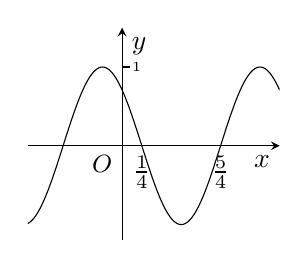
\begin{tikzpicture}
        \node[below left](O) at(0,0) {\small$\bm{O}$};
        \draw(0,1)node[right]{\tiny$1$}--(0.1,1);
        \clip(-1.2,-1.2) rectangle (2,1.5);
        \draw[->,>=stealth](-1.2,0)--(2,0) node[below left] (x){$x$};
        \draw[->,>=stealth](0,-1.2)--(0,1.5) node[below right] (y){$y$};
        \draw[domain=-1.2:2,samples=1000] plot(\x,{cos((pi*(\x)+1/4*pi) r)});
        \node[below] (A)at (0.25,0){$\frac{1}{4}$};
        \node[below] (B)at (1.25,0){$\frac{5}{4}$};
      \end{tikzpicture}
      \end{center}
      \twochx{$ \left(k\pi-\dfrac{1}{4},k\pi+\dfrac{3}{4}\right),k\inZ$}
        {$ \left(2k\pi-\dfrac{1}{4},2k\pi+\dfrac{3}{4}\right),k\inZ$}
        {$ \left(k-\dfrac{1}{4},k+\dfrac{3}{4}\right),k\inZ$}
        {$\left(2k-\dfrac{1}{4},2k+\dfrac{3}{4}\right),k\inZ $}
  \end{exercise}
\section{三角函数模型的简单应用-}
 \fz[12]
$f(x0)=d d$\fz[4]
\section{课后作业}
  \begin{exercise}

  \end{exercise}
\stopexercise
\section{参考答案}
\printanswer

% \Topic{三角函数单元复习}
  \Teach{}
  \Grade{高一}
  % \Name{郑皓天}\FirstTime{20181207}\CurrentTime{20181207}
  % \Name{林叶}\FirstTime{20180908}\CurrentTime{20181125}
  %\Name{1v2}\FirstTime{20181028}\CurrentTime{20181117}
  % \Name{林叶}\FirstTime{20180908}\CurrentTime{20181125}
  % \Name{郭文镔}\FirstTime{20181111}\CurrentTime{20181117}
  % \Name{马灿威}\FirstTime{20181111}\CurrentTime{20181111}
  \newtheorem*{Theorem}{定理}
  \makefront
\vspace{-1.5em}
\startexercise
% \begin{exercise}{\heiti 课前检测}\\
% \end{exercise}
\section{习题}
  % \begin{description}
  %   \item [label]
  % \end{description}
  \begin{exercise}
    \item%高中数学习题解法辞典.pdf 2-1-8
      已知$\abs{\cos \theta}\leqslant \abs{\sin\theta}$,则$\theta$的取值范围是\tk.
      \begin{answer}
        $\Bigl[k\piup+\dfrac{\piup}4,k\piup+\dfrac{3\piup}4\Bigr],k\in\mathbb{Z}$
      \end{answer}
    \item%高中数学习题解法辞典.pdf 2-1-19
      已知$\sin\Bigl(\dfrac{\piup}2+2x\Bigr)=-\dfrac12$,则$x=$\tk.
      \begin{answer}
        k\piup\pm\dfrac{\piup}3(k\in\mathbb{Z})
      \end{answer}
    \item%高中数学习题解法辞典.pdf 2-2-4
      函数$y=\sqrt{25-x^2}+\lg\sin\Bigl(x+\dfrac{\piup}3\Bigr)$的定义域为\tk.
      \begin{answer}
        $\Bigl[-5,-\dfrac{4\piup}3\Bigr)\bigcup\Bigl(-\dfrac{\piup}3,\dfrac{2\piup}3\Bigr)$
      \end{answer}
    \item%LaTeX-master/sanjiaohanshu/sanjiaohanshu-gaokao.tex 4
      函数$f(x)=\cos(\omega x+\varphi)$的部分图象如图所示,则$f(x)$的单调递减区间为\xz
      \begin{minipage}[b]{0.8\linewidth}
        \vspace{2.5em}
        \xx{$\Bigl(k\piup-\dfrac{1}{4},k\piup+\dfrac{3}{4}\Bigr),k\in\mathbb{Z}$}
          {$ \Bigl(2k\piup-\dfrac{1}{4},2k\piup+\dfrac{3}{4}\Bigr),k\in\mathbb{Z}$}
          {$ \Bigl(k-\dfrac{1}{4},k+\dfrac{3}{4}\Bigr),k\in\mathbb{Z}$}
          {$\Bigl(2k-\dfrac{1}{4},2k+\dfrac{3}{4}\Bigr),k\in\mathbb{Z} $}
      \end{minipage}\hfill
      \begin{minipage}[h]{0.2\linewidth}
        \vspace{-3cm}
        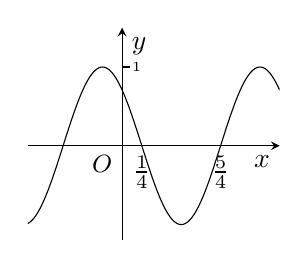
\begin{tikzpicture}
          \node[below left](O) at(0,0) {\small$\bm{O}$};
          \draw(0,1)node[right]{\tiny$1$}--(0.1,1);
          \clip(-1.2,-1.2) rectangle (2,1.5);
          \draw[->,>=stealth](-1.2,0)--(2,0) node[below left] (x){$x$};
          \draw[->,>=stealth](0,-1.2)--(0,1.5) node[below right] (y){$y$};
          \draw[domain=-1.2:2,samples=1000] plot(\x,{cos((pi*(\x)+1/4*pi) r)});
          \node[below] (A)at (0.25,0){$\frac{1}{4}$};
          \node[below] (B)at (1.25,0){$\frac{5}{4}$};
        \end{tikzpicture}
      \end{minipage}
      \begin{answer}
        D
      \end{answer}
    \item%《习题化知识清单》P72知识2-2
      不等式$\tan x>a$在$x\in\Bigl(-\dfrac{\piup}4,\dfrac{\piup}2 \Bigr)$上恒成立,则$a$的取值范围是\xz
      \xx{$(-\infty,-1]$}
        {$(-\infty,-1)$}
        {$(-\infty,1]$}
        {$(-\infty,1]$}
      \begin{answer}
        A
      \end{answer}
    \item%福州三中中学2015-2016学年高一数学第二学期期末检测.docx-9
      (福州三中中学2015-2016学年高一数学第二学期期末检测9)将函数$y=\sin\Bigl(x-\dfrac{\piup}3\Bigr)$的图像上所有点的横坐标伸长到原来的2倍(纵坐标不变),再将所得的图像向左平移$\dfrac{\piup}3$个单位,得到的函数图像对应的解析式是\xz
      \xx{$y=\sin\dfrac x2$}
        {$y=\sin\Bigl(\dfrac x2-\dfrac{\piup}2\Bigr)$}
        {$y=\sin\Bigl(\dfrac{x}2-\dfrac{\piup}6\Bigr)$}
        {$y=\sin\Bigl(2x-\dfrac{\piup}6\Bigr)$}
      \begin{answer}
        C
      \end{answer}
    \item%《习题化知识清单》P73易混清单例
      函数$y=2\sin\Bigl(\dfrac{\piup}3-2x \Bigr)$的单调增区间为\tk.
      \begin{answer}
        $\Bigl[k\piup+\dfrac{5\piup}{12},k\piup+\dfrac{11\piup}{12} \Bigr],k\in\mathbb{Z}$
      \end{answer}
    \item%《习题化知识清单》P72例1
      函数$\dfrac{\sin x+2}{\sin x+1},x\in\Bigl[0,\dfrac{\piup}2\Bigr]$的值域为\tk.
      \begin{answer}
        $\Bigl[\dfrac32,2\Bigr]$
      \end{answer}
    \item%LaTeX-master/sanjiaohanshu/gaokaosection.tex 31
      把函数$ y=\sin 2x $的图象沿$x$轴向左平移$ \dfrac{\piup}{6} $个单位,纵坐标伸长到原来的2倍(横坐标不变)后得到函数$ y=f(x) $的图象,对于函数$ y=f(x) $有以下四个判断:\\
      \ding{192} 该函数的解析式为$ y=2\sin \Bigl(2x+\dfrac{\piup}{6}\Bigr) $;\\
      \ding{193} 该函数图象关于点$ \Bigl(\dfrac{\piup}{3},0\Bigr) $对称;\\
      \ding{194} 该函数在$ \Bigl[0,\dfrac{\piup}{6}\Bigr] $上是增函数;\\
      \ding{195} 若函数$ y=f(x)+a $在$ \Bigl[0,\dfrac{\piup}{2}\Bigr] $上的最小值为$ \sqrt{3},\  $则$ a=2\sqrt{3} .$\\
      其中,正确判断的序号是\tk.
      \begin{answer}
        \circled{2}\circled{4}
      \end{answer}
    \item%福州格致中学2015-2016学年高一数学第二学期期末检测.docx-22
      (福州格致中学2015-2016学年高一数学第二学期期末检测22)已知函数$f(x)=A\sin(\omega x+\varphi)+B (A>0,\omega>0)$的一系列对应值如下表:
      \begin{center}
        \renewcommand{\arraystretch}{1.4}
        \begin{tabular}{|*{8}{c|}}
          \hline
            $x$
            &$-\dfrac{\piup}6$
            &$-\dfrac{\piup}3$
            &$-\dfrac{5\piup}6$
            &$-\dfrac{4\piup}3$
            &$-\dfrac{11\piup}6$
            &$-\dfrac{7\piup}3$
            &$-\dfrac{17\piup}6$\\
          \hline
            $y$
            &$-1$
            &$1$
            &$3$
            &$1$
            &$-1$
            &$1$
            &$3$\\
          \hline
        \end{tabular}\\
      \end{center}
      (1)根据表格提供的数据求函数$f(x)$的一个解析式;\\
      (2)根据(1)的结果:\\
      \;(i)当$x\in\Bigl[0,\dfrac{\piup}3\Bigr]$时,方程$f(3x)=m$恰有两个不同的解,求实数$m$的取值范围;\\
      \;(ii)若是$\alpha,\beta$是锐角三角形的两个内角,试比较$f(\sin \alpha)$与$f(\cos \beta)$的大小.
      \begin{answer}
        (1)$f(x)=2\sin\Bigl(x-\dfrac{\piup}3\Bigr)+1$;(2)(i)$[\sqrt{3}+1,3)$;(ii)易得$f(x)$在$[-\dfrac{\piup}6,\dfrac{5\piup}6]$上单调递增,故$f(x)$在$[0,1]$上单调递增;又$0<\dfrac{\piup}2-\beta<\alpha<\dfrac{\piup}2$,从而$\sin\alpha>\sin(\dfrac{\piup}2-\beta)=\cos\beta$,于是$f(\sin \alpha)>f(\cos \beta)$
      \end{answer}
    \vspace{6.5cm}
    \item%高中数学习题解法辞典.pdf 2-2-9
      已知函数$y=f(x)$的定义域为$\mathbb{R}$,若$f(x+2)=-f(x)$,且当$-1\leqslant x\leqslant 1$时,$f(x)=x$,求证:\\
      (1)函数$y=f(x)$是最小正周期为4的周期函数;\\
      (2)函数$y=f(x)$是奇函数;\\
      (3)当$x\in[4k-1,4k+1](k\in\mathbb{Z})$时,$y=f(x)$是增函数;当$x\in[4k+1,4k+3](k\in\mathbb{Z})$时,$y=f(x)$是减函数.
      % \begin{answer}
      %
      % \end{answer}
  \end{exercise}

\newpage
\section{课后作业}
  \begin{exercise}
    \item%高中数学习题解法辞典.pdf 2-1-74
      已知$1+\sin^2x=\cos x$,则$x=$\tk.
      \begin{answer}
        $2k\piup(k\in\mathbb{Z})$
      \end{answer}
    \item%《习题化知识清单》P72方法2-1
      函数$\abs{\sin x}$的一个单调区间是\xz
      \xx{$\Bigl(\dfrac{\piup}2,\piup\Bigr)$}
        {$\Bigl(\piup,2\piup\Bigr)$}
        {$\Bigl(\piup,\dfrac{3\piup}2\Bigr)$}
        {$\Bigl(0,\piup\Bigr)$}
      \begin{answer}
        C
      \end{answer}
    \item%LaTeX-master/sanjiaohanshu/gaokaosection.tex 13
       已知函数$f(x)=\Bigg\{\begin{aligned}
      \sin(x+a),x\le 0\\\cos (x+b),x>0
      \end{aligned}$是偶函数,则下列结论可能成立的是\xz
       \xx{$ a=\dfrac{\piup}{4},b=-\dfrac{\piup}{4}$}
        {$ a=\dfrac{2\piup}{3},b=\dfrac{\piup}{6}$}
        {$a=\dfrac{\piup}{3},b=\dfrac{\piup}{6} $}
        {$ a=\dfrac{5\piup}{6},b=\dfrac{2\piup}{3}$}
      \begin{answer}
        C
      \end{answer}
    \item%《习题化知识清单》P77单元检测10
      定义在$\mathbb{R}$上的偶函数$f(x)$满足$f(x+1)=-\dfrac2{f(x)}(f(x)\neq0)$,且在区间$(2013,2014)$上单调递增.已知$\alpha,\beta$是锐角三角形的两个内角,则$f(\sin\alpha),f(\cos\beta)$的大小关系是\xz
      \xx{$f(\sin\alpha)<f(\cos\beta)$}
        {$f(\sin\alpha)>f(\cos\beta)$}
        {$f(\sin\alpha)=f(\cos\beta)$}
        {以上情况均有可能}
    \item%《习题化知识清单》P72知识3-3
      若函数$y=2\cos(2x+\varphi)$是偶函数,且在$\Bigl(0,\dfrac{\piup}4\Bigr)$上是增函数,则实数$\varphi$可能是\xz
      \xx{$-\dfrac{\piup}2$}
        {0}
        {{$\dfrac{\piup}2$}}
        {$\piup$}
      \begin{answer}
        D
      \end{answer}
    \item%高中数学习题解法辞典.pdf 2-1-74
      比较$\sin 3$,$\cos 3$,$\tan 0.8$的大小关系为\tk.
      \begin{answer}
        $\tan 0.8>\sin 3>\cos 3$
      \end{answer}
    \item%LaTeX-master/sanjiaohanshu/gaokaosection.tex 26
      已知函数$f(x)=\sin (2x+\varphi)$,若$    f\Bigl(\dfrac{\piup}{12}\Bigr)-f\Bigl(-\dfrac{5\piup}{12}\Bigr)=2 $,则函数$f(x)$的单调增区间为\tk.
      \begin{answer}
        $\Bigl[k\piup-\dfrac{5\piup}{12},k\piup+\dfrac{\piup}{12}\Bigr],k\in\mathbb{Z}$
      \end{answer}
    \item%函数y=Asin(ωx+φ)的图象及简单应用P11.9
      若$f(x)=\cos\Bigl(2x+\dfrac{\piup}3+\varphi\Bigr)$$(\abs{\varphi}<\dfrac{\piup}2)$是奇函数,则$\varphi=$\tk.
      \begin{answer}
        $\dfrac{\piup}6$
      \end{answer}
    \item%《习题化知识清单》P77单元检测12
      设$\omega>0$,若函数$f(x)=2\sin \omega x(\omega>0)$在区间$\Bigl[-\dfrac{\piup}3,\dfrac{\piup}4 \Bigr]$上单调递增,则$\omega$取值范围是\tk.
      \begin{answer}
        $\Bigl(0,\dfrac32\Bigr]$
      \end{answer}
    \item%高中数学习题解法辞典.pdf 2-2-1
      已知函数$f(x)=A\sin(\omega x+\varphi)(A,\omega,\varphi\text{为常数},\omega>0)$的图像上相邻两个最高点的坐标分别是$\Bigl(\dfrac{\piup}{12},2\Bigr)$,$\Bigl(\dfrac{13\piup}{12},2\Bigr)$.\\
      (1) 求函数$f(x)$的一个表达式;\\
      (2)画出函数$f(x)$在长度为一个周期的闭区间上的简图;\\
      (3)说明经过怎样的变换,可以由$y=\sin x$的图像得到$y=f(x)$的图像.
      \begin{answer}
        (1)$y=2\sin\Bigl(2x+\dfrac{\piup}3\Bigr)(\varphi=k\piup-\dfrac{2\piup}3$即可);(2)略;(3)将$y=\sin x$图像上所有点向左平移$\dfrac{\piup}3$个单位得到$y=\sin \Bigl(x+\dfrac{\piup}3\Bigr)$的图像;再把$y=\sin \Bigl(x+\dfrac{\piup}3\Bigr)$的图像上所有点的横坐标缩短到原来的$\dfrac12$(纵坐标不变),得到$y=\sin \Bigl(2x+\dfrac{\piup}3\Bigr)$的图像;最后把$y=\sin \Bigl(2x+\dfrac{\piup}3\Bigr)$的图像上所有点的纵坐标伸长到原来的2倍(横坐标不变),即可得到函数$y=f(x)$的图像.
      \end{answer}
    \vspace{6cm}
    \item%函数y=Asin(ωx+φ)的图象及简单应用P11.14
      已知曲线$y=A\sin(\omega x+\varphi)$$(A>0,\omega>0,\abs{\varphi}\leqslant\dfrac{\piup}2)$上最高点为$(2,\sqrt{2})$,该最高点与相邻的最低点间的曲线与$x$轴交于点$(6,0)$.\\
      (1)该函数的解析式;\\
      (2)该函数在$x\in[-6,0]$上的值域.
      \begin{answer}
        (1)$y=\sqrt{2}\sin\Bigl(\dfrac{\piup}8x+\dfrac{\piup}4\Bigr)$;
        (2)$[-\sqrt{2},0]$
      \end{answer}
    \vspace{5cm}
    \item%高中数学习题解法辞典.pdf 2-2-44
      已知函数$f(x)=2\sin\Bigl(\omega x+\dfrac{\piup}6\Bigr)(\omega>0)$,\\
      (1)求$f(x)$的最大值$M$,最小值$m$以及最小正周期$T$;\\
      (2)试求最小正整数$\omega$,使得自变量$x$在任意两个整数间(包括整数本身)变化时,函数$f(x)$至少有一个值是$M$,另一个值是$m$.
      \begin{answer}
        (1)$M=3,m=-1,T=\dfrac{2\piup}{\omega}$;(2)$\dfrac{2\piup}{\omega}\leqslant 1$,$\omega=7$
      \end{answer}
    \vspace{6cm}
    \item%高中数学习题解法辞典.pdf 2-2-45
      求证:(1)$f(x)=\sin x\cos x$的最小正周期为$\piup$;\\
      (2)若函数$y=f(x)(x\in\mathbb{R})$的最小正周期为$T$,则$f(kx)(k>0)$的最小正周期为$\dfrac{T}k$.
      \begin{answer}
        (1)(提示:若$0<T<\piup$,令$x=0$,得$T=\dfrac{\piup}2$,不符);(2)(提示:$f\biggl[k\Bigl(x+\dfrac{T}k\Bigr)\biggr]=f(kx+T)=f(kx)$)
      \end{answer}
  \end{exercise}
\stopexercise

\newpage
\section{部分参考答案}
\begin{multicols}{2}
  \printanswer
\end{multicols}

% sty文件使用 \RequirePackage{latexexercise0}
% 主文件使用 \documentclass[a3paper,twocolumn,2twoside,landscape,12pt,UTF8]{ctexart}
% \hspace{3cm}\\
% \vspace{0.5cm}
% \part{\centering{\heiti \xiaoer 福州清大教育2018-2019学年高一数学期末考模拟卷}}\\
\twocolumn
\part{\mbox{\heiti \xiaoer 福州清大教育2018-2019学年高一数学期末考模拟卷}}
  % \vspace{-1.5cm}
  \centering{\heiti \erhao 高一数学\quad 必修四}\\
  \centering{\wuhao (考试时间:120分钟,满分:150分,另附加分30分)}\\
  \vspace{-1.6em}
  \startexercise
  \begin{exercise}
  \section{选择题(本大题共12小题,每小题5分,共60分.每题有且只有一个选项是正确的,请把答案填在答卷相应位置上)}
    \item%福州三中2016-2017学年第二学期高一数学期末考试-1【弧度制与角度制】
      关于角度制与弧度制的等式,正确的是\xz
      \xx{$\piup=1\rm{rad}$}
        {$\piup=180$}
        {$1^{\degree}=\dfrac{180}{\piup}\rm{rad}$}
        {$1\rm{rad}=\Bigl(\dfrac{180}{\piup}\Bigr)^\degree$}
      \begin{answer}
        D
      \end{answer}
    \item%格致中学2015-2016学年第四学段高一期末考试-3【任意角三角函数】
      已知$\tan\alpha=-\sqrt3,0<\alpha<\piup$,那么$\cos\alpha-\sin\alpha$的值是\xz
      \xx{$-\dfrac{1+\sqrt3}2$}
        {$\dfrac{-1+\sqrt3}2$}
        {$\dfrac{1-\sqrt3}2$}
        {$\dfrac{1+\sqrt3}2$}
      \begin{answer}
        A
      \end{answer}
    \item%LaTeX-master/xiangliang/xiangliangsorting.tex 练习P7-10【向量共线、线性运算】
      设$ D $为$\triangle ABC$所在平面内一点,$ \vv{BC}=3\vv{CD} $,则\xz
      \xx{$ \vv{AD}=-\dfrac{1}{3}\vv{AB}+\dfrac{4}{3}\vv{AC}$}
        {$ \vv{AD}=\dfrac{1}{3}\vv{AB}-\dfrac{4}{3}\vv{AC}$}
        {$ \vv{AD}=\dfrac{4}{3}\vv{AB}+\dfrac{1}{3}\vv{AC}$}
        {$ \vv{AD}=\dfrac{4}{3}\vv{AB}-\dfrac{1}{3}\vv{AC}$}
      \begin{answer}
        A
      \end{answer}
    \item%LaTeX-master/2018/qimo.tex-7【Asin(\omega x+\varphi)】
      函数$f(x)=2\sin\left(\omega x+\varphi\right)\left(\omega>0,\abs{\varphi}<\dfrac{\pi}{2}\right)$的部分图象如图所示,则$ \omega,\varphi $的值分别是\xz
      \begin{minipage}[b]{0.7\linewidth}
        \vspace{1.5cm}
        \xx{$ 2,-\dfrac{\pi}{3}$}{$2,-\dfrac{\pi}{6} $}{$4,-\dfrac{\pi}{6} $}{$ 4,\dfrac{\pi}{3}$}
      \end{minipage}\hfill
      \begin{minipage}[h]{0.3\linewidth}
        \vspace{-1cm}
        \begin{tikzpicture}[>=latex,scale=1]
          \tikzmath{
            \a = 5*pi/12;
            \b=11*pi/12;
          }
          \draw[->](-1,0)--(4,0) node[below](x){$x$};
          \draw[->](0,-2.3)--(0,2.3) node[left](y){$y$};
          \node[below left](O) at(0,0){$\small O$};
          \draw[domain=0:pi,samples=1000] plot (\x,{2*sin((2*(\x)-pi/3) r)});
          \draw[dashed] (0,2)node[left](a){$2$}-|(\a,0)node[below](a1){$\dfrac{5\pi}{12}$} ;;
          \draw[dashed](0,-2)node[left](b){$-2$}-|(\b,0)node[above](b1){$\dfrac{11\pi}{12}$} ;
          %\draw[dashed] (0,2)-|($(5*pi/12,0)$);
        \end{tikzpicture}
      \end{minipage}
      \begin{answer}
        A
      \end{answer}
    \item%《习题化知识清单》P85方法3-4.1【向量夹角垂直】
      向量$\bm a=(1,-2),\bm b=(2,1)$,则\xz
      \xx{$\bm a\varparallel \bm b$}
        {$\bm a\perp \bm b$}
        {$\bm a$与$\bm b$的夹角为$60\degree$}
        {$\bm a$与$\bm b$的夹角为$30\degree$}
      \begin{answer}
        B
      \end{answer}
    \item%《习题化知识清单》P84知识5-23【数量积应用,三角形五心】
      点$O$是$\triangle{ABC}$所在平面上的一点,且满足$\vv{OA}\cdot\vv{OB}=\vv{OB}\cdot\vv{OC}=\vv{OA}\cdot\vv{OC}$,则点$O$是$\triangle{ABC}$的\xz
        \xx{重心}
          {垂心}
          {内心}
          {外心}
      \begin{answer}
        B
      \end{answer}
    \item%《习题化知识清单》P71知识-4【诱导公式】
      已知$\sin{\Bigl(\dfrac{\piup}3+\alpha\Bigr)}=-\dfrac{5}{13}$,则$\cos{\Bigl(\dfrac{\piup}6-\alpha \Bigr)}=$\xz
      \xx{$-\dfrac{5}{12}$}
        {$\dfrac{5}{13}$}
        {$-\dfrac{5}{13}$}
        {$\dfrac{1}{5}$}
      \begin{answer}
        C
      \end{answer}
    \item%《习题化知识清单》P89知识3-3【三角恒等变换,综合】
      若$\alpha\in(0,\piup)$,且$\cos\alpha+\sin\alpha=-\dfrac{1}{3}$,则$\cos{2\alpha}$等于\xz
        \xx{$\dfrac{17}9$}
          {$\pm\dfrac{17}9$}
          {$-\dfrac{17}9$}
          {$\dfrac{17}3$}
      \begin{answer}
        A
      \end{answer}
    \item%《习题化知识清单》P90单元检测10【数量积;三角恒等变换,综合】
      已知向量$\bm a=\Bigl(\cos\dfrac{3x}2,\sin\dfrac{3x}2\Bigr)$,$\bm b=\Bigl(\cos\dfrac{x}2,-\sin\dfrac{x}2\Bigr)$,且$x\in\Bigl[0,\dfrac{\piup}2\Bigr]$,
      若$\abs{\bm a+\bm b}=2\bm a\cdot\bm b$,则$\sin{2x}+\tan{x}=$\xz
      \xx{$-1$}{$0$}{$2$}{$-2$}
      \begin{answer}
        B
      \end{answer}
    \item%《习题化知识清单》P75方法2.3【三角函数图像】
      设函数$f(x)=\sin{\Bigl(2x+\dfrac{\piup}3\Bigr)}$,则下列结论正确的是\xz
      \xx{$f(x)$的图像关于直线$x=\dfrac{\piup}3$对称}
        {$f(x)$的图像关于点$\Bigl(-\dfrac{\piup}4,0\Bigr)$对称}
        {把$f(x)$的图像向左平移$\dfrac{\piup}{12}$个单位长度,得到一个偶函数的图像}
        {$f(x)$的最小正周期为$\piup$,且在$\Bigl[0,\dfrac{\piup}6 \Bigr]
        $上为增函数}
      \begin{answer}
        C
      \end{answer}
    \item%《习题化知识清单》P90单元检测8【向量投影】
      在平面直角坐标系中,$AB=CD$,$A(0,3)$,$B(-4,0)$,$C(a,-1)(a>0)$,则向量$\vv{BC}$在$\vv{AB}$上的投影为\xz
        \xx{$-5$}
          {$-3$}
          {$3$}
          {$5$}
      \begin{answer}
        A
      \end{answer}
    \item%《习题化知识清单》P90单元检测9【三角恒等变换,二次方程】
      已知$\tan\alpha$,$\tan\beta$是方程$x^2-3x-5=0$的两根,则$\tan{2(\alpha+\beta)}$的值为\xz
        \xx{$-\dfrac{24}{25}$}
          {$\dfrac{24}7$}
          {$-\dfrac{4}{5}$}
          {$-\dfrac{4}{3}$}
      \begin{answer}
        D
      \end{answer}
    \item%《高中数学竞赛培优教程+一试(李名德 主编)》.pdf P122-5.2-3
      (附加题,5分)
      已知正方形$PQRS$对角线交点为$M$,坐标原点$O$不在正方形内部,$\vv{OP}=(0,3)$,$\vv{OS}=(4,0)$,则向量$\vv{RM}$为\xz
      \xx{$\Bigl(-\dfrac{7}{2},-\dfrac{1}{2}\Bigr)$}
        {$\Bigl(\dfrac{7}{2},\dfrac{1}{2}\Bigr)$}
        {$(7,4)$}
        {$\Bigl(\dfrac{7}{2},\dfrac{7}{2}\Bigr)$}
      \begin{answer}
        A
      \end{answer}
    \item%《高中数学竞赛培优教程+一试(李名德 主编)》.pdf P92-4.1-4
      (附加题,5分)
      已知$\theta\in[0,\piup]$,$f(x)=\sin{(\cos\theta)}$的最大值为$a$,最小值为$b$,$g(\theta)=\cos{(\sin\theta)}$的最大值为$c$,最小值为$d$,则$a,b,c,d$从小到大的顺序是\xz
      \xx{$b<d<a<c$}
        {$d<b<c<a$}
        {$b<d<c<a$}
        {$d<b<a<c$}
      \begin{answer}
        A
      \end{answer}
  \section{填空题(本大题共4小题,每小题5分,共20分)}
    \item%《习题化知识清单》P84方法1-1【向量夹角,参数】
       已知$\abs{\bm a}=1,\abs{\bm b}=2$,$\bm a$与$\bm b$的夹角为$120\degree$,则使$\bm a+k\bm b$与$k\bm a+\bm b$的夹角为锐角的实数$k$的取值范围是\tk[5].
      \begin{answer}
        $\Bigl(\dfrac{5-\sqrt{21}}2,1\Bigr)\bigcup\Bigl(1,\dfrac{5+\sqrt{21}}2\Bigr)$
      \end{answer}
    \item%《习题化知识清单》P70方法3.2【同角三角函数关系化简】
      已知$\sin\alpha\cos\alpha=-\dfrac{12}{25}$,$\alpha\in\Bigl(-\dfrac{\piup}4,0\Bigr)$,则$\sin\alpha+\cos\alpha=$\tk.
      \begin{answer}
        $\dfrac{1}{5}$
      \end{answer}
    \item%《习题化知识清单》P85方法4-5.2【数量积,数形结合】
       已知正方形$ABCD$的边长为1,点$E$是$AB$边上的动点,则$\vv{DE}\cdot\vv{DC}$的最大值为\tk.
       \begin{answer}
         1
       \end{answer}
    \item%《习题化知识清单》P89方法1-1【三角恒等变换,函数性质】
       已知函数$f(x)=\dfrac{(\sin x-\cos x)\sin {2x}}{\sin x}$,则$f(x)$的单调递减区间为\tk[6].
      \begin{answer}
        $\Bigl[k\piup+\dfrac{3\piup}8,k\piup+\dfrac{7\piup}8\Bigr](k\in\mathbb{Z})$
      \end{answer}
    \item%《高中数学奥林匹克竞赛解题方法大全(周沛耕 主编)》.pdf P93例3
      (附加题,5分)
      $\sqrt3\tan{18\degree}+\tan{18\degree}\tan{12\degree}+\sqrt3\tan{12\degree}=$\tk.
      \begin{answer}
        1
      \end{answer}
  % \clearpage
  \section{解答题(本大题共有6个小题,共70分. 解答应写出文字说明、演算步骤或证明过程)}
    \item
      (本小题满分10分)求值:\\
      已知$\abs{\vv a}=\sqrt2,\abs{\vv{\mathstrut b}}=1$
      (1)若$\vv a,\vv b$的夹角$\theta$为$45\degree$,求$\abs{\vv{\mathstrut a}-\vv{\mathstrut b}}$;\\
      (2)若$(\vv{\mathstrut a}-\vv{\mathstrut b})\perp \vv{\mathstrut b}$,求$\vv{\mathstrut a}$与$\vv{\mathstrut b}$的夹角$\theta$.
      \begin{answer}
        解:(1) $\abs{\vv a-\vv b}=\sqrt{\vv a^2-2\vv a\!\cdot\!\vv b+\vv b^2}=\sqrt{2-2\times\sqrt2\times1\times\dfrac{\sqrt2}2+1}=1$\fz[5]
        (2)$\because(\vv a-\vv b)\perp\vv b$,\\
        $\therefore(\vv a-\vv b)\cdot\vv b=\vv a\cdot\vv b-\vv b^2=\sqrt2\times1\times\cos\theta-1=0$,\\
        $\therefore\cos\theta=\dfrac{\sqrt2}2(0\le\theta\le\piup)$,$\therefore\theta=\dfrac{\piup}4.$\fz[10]
      \end{answer}
    \vspace{3cm}
    \clearpage
    \item
      (本小题满分12分)\par
      (1)化简:$\dfrac{\cos{\Bigl(\alpha-\dfrac{\piup}2\Bigr)}}{\sin{\Bigl(\dfrac{5\piup}2+\alpha\Bigr)}}\cdot\sin{(\alpha-2\piup)}\cdot\cos{(\piup-\alpha)}$;\\
      (2)已知$\tan{a}=-2$,求$\dfrac{\sin{2a}-\cos^2{a}}{2+\cos{2a}}$的值.
      \begin{answer}
      解:(1)$\text{原式}=\dfrac{\sin\alpha}{\cos\alpha}\cdot\sin\alpha\cdot(-\cos\alpha)=-\sin^2\alpha$;\\
      (2)$\because\tan\alpha=-2$,
      $\therefore\text{原式}=\dfrac{2\sin\alpha\cdot\cos\alpha-\cos^2\alpha}{2\cos^2\alpha+1}
      =\dfrac{2\sin\alpha\cdot\cos\alpha-\cos^2\alpha}{3\cos^2\alpha+\sin^2\alpha}
      =\dfrac{\dfrac{2\sin\alpha\cdot\cos\alpha-\cos^2\alpha}{\cos^2\alpha}}{\dfrac{3\cos^2\alpha+\sin^2\alpha}{\cos^2\alpha}}
      =\dfrac{2\tan\alpha-1}{3+\tan^2\alpha}=\dfrac{2\times(-2)-1}{3+(-2)^2}
      =-\dfrac{5}{7}.$
      \end{answer}
    \vspace{3cm}
    \item
      (本小题满分12分)\\
      设函数$f(x)=\bm a\cdot\bm b$,其中向量$\bm a=(\cos x,1)$,$\bm b=\bigl(\cos x,\sqrt3\sin x\cos x\bigr)$,$x\in\mathbb{R}$.\\
      (1)求函数$f(x)$的解析式;\\
      (2)求满足$f(x)\leqslant0$的$x$的集合;\\
      (3)函数$y=\sin x$的图像可由函数$y=f(x)$的图像经过怎样的变换得到?\\
      \begin{answer}
        解:(1)$f(x)=\bm a\cdot\bm b
        =\cos^2x+\sqrt3\sin x\cos x
        =\dfrac{\cos{2x}+1}2+\dfrac{\sqrt3}{2}\sin{2x}
        =\sin{\Bigl(2x+\dfrac{\piup}6\Bigr)}+\dfrac12.$\\
        (2)$\because f(x)\leqslant0$,
        $\therefore \sin{\Bigl(2x+\dfrac{\piup}6\Bigr)}\leqslant-\dfrac12.$\\
        又$\because$不等式$\sin x\leqslant-\dfrac12$的解集为$\Bigl[2k\piup-\dfrac{5\piup}6,2k\piup-\dfrac{\piup}6\Bigr],k\in\mathbb{Z}.$\\
        $\therefore 2k\piup-\dfrac{5\piup}6 \leqslant 2x+\dfrac{\piup}6 \leqslant 2k\piup-\dfrac{\piup}6$.\\
        解得:$k\piup-\dfrac{\piup}2 \leqslant x \leqslant k\piup-\dfrac{\piup}6$
        即:函数$f(x)\leqslant0$的$x$的解集为$\Bigl\{x\Bigm| k\piup-\dfrac{\piup}2 \leqslant x \leqslant k\piup-\dfrac{\piup}6,k\in\mathbb{Z}\Bigr\}$.\\
        (3)函数$y=\sin x$的图像可由函数$y=f(x)$的图像经过以下步骤变换得到:\\
        $\circled{1}$向下平移$\dfrac12$个单位,得到函数$y=\sin{\Bigl(2x+\dfrac{\piup}6\Bigr)}$的图像;\\
        $\circled{2}$向右平移$\dfrac{\piup}{12}$个单位,得到函数$y=\sin {2x}$的图像;\\
        $\circled{3}$横坐标伸长2倍,得到函数$y=\sin x$的图像.
      \end{answer}
    \vspace{3.6cm}
    \item
      (本小题满分12分)\\
      已知函数$f(x)=2\sin^2{\Bigl(\dfrac{\piup}4+x\Bigr)}+\sqrt3\cos{2x}$.\\
      (1)求函数$f(x)$的最小正周期和对称轴方程;\\
      (2)若关于$x$的方程$f(x)-m=2$在$x\in\Bigl[0,\dfrac{\piup}2\Bigr]$上有两个不同的解,求实数$m$的取值范围.\\
      \begin{answer}
        【分析】(1)利用三角函数的倍角公式以及辅助角公式将函数进行化简即可求最小正周期和对称轴方程;\\
        (2)求出函数$f(x)$在$x\in\Bigl[0,\dfrac{\piup}2\Bigr]$的取值情况,利用数形结合即可得到结论.\\
        【解答】解:(1)由$f(x)=2\sin^2{\Bigl(\dfrac{\piup}4+x\Bigr)}+\sqrt3\cos{2x}
        =1-\cos{\Bigl(\dfrac{\piup}2+2x\Bigr)}+\sqrt3\cos{2x}
        =1+\sin{2x}+\sqrt3\cos{2x}=1+2\sin{\Bigl(\dfrac{\piup}3+2x\Bigr)}$,\\
        $\because \omega=2$,$\therefore$函数$f(x)$的最小正周期为$\piup$.\\
        由$2x+\dfrac{\piup}3=\dfrac{\piup}2+k\piup,k\in\mathbb{Z}$得:$x=\dfrac{\piup}{12}+\dfrac12k\piup,{k\in\mathbb{Z}}$,\\
        故函数$f(x)$的对称轴方程为:$x=\dfrac{\piup}{12}+\dfrac12k\piup,{k\in\mathbb{Z}}$.\\
        (2)由$f(x)-m=2$得$f(x)=m+2$,\\
        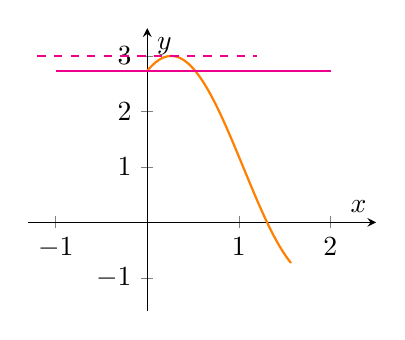
\begin{tikzpicture}[declare function={f(\k)=1+2*sin(deg(2*\k+pi/3));}]
          \tikzset{elegant/.style={smooth,thick,samples=50,magenta}}
          \begin{axis}[axis x line=middle,
                 axis y line=middle,
                 xmin=-1.3,xmax=2.5,
                 ymin=-1.6,ymax=3.5,
                 xstep=1,ystep=1,
                 ytick distance=1,
                 ylabel=$y$,
                 xlabel=$x$]
                \addplot[elegant,orange,domain=0:pi/2]{f(x)};
                \addplot[elegant,dashed,domain=-1.2:1.2]{3};
                \addplot[elegant,domain=-1:2]{2.732};
          \end{axis}
        \end{tikzpicture}
        当${x\in\Bigl[0,\dfrac{\piup}2\Bigr]}$时,$2x+\dfrac{\piup}3\in\Bigl[\dfrac{\piup}3,\dfrac{4\piup}3\Bigr]$,\\
        由图象得$f(0)=1+2\sin{\dfrac{\piup}3}=1+\sqrt3$,\\
        函数$f(x)$的最大值为$1+2=3$,\\
        $\therefore$要使方程$f(x)-m=2$在$x\in\Bigl[0,\dfrac{\piup}2\Bigr]$上有两个不同的解,
        则$f(x)=m+2$在$x\in\Bigl[0,\dfrac{\piup}2\Bigr]$上有两个不同的解,\\
        即函数$f(x)$和$y=m+2$在$x\in\Bigl[0,\dfrac{\piup}2\Bigr]$上有两个不同的交点,\\
        即$1+\sqrt3\leqslant m+2<3$,\\
        即 $\sqrt3-1\leqslant m<1$.
      \end{answer}
    \vspace{3.6cm}
    \item
      (本小题满分12分)\\
      已知向量$\bm a=\Bigl(\dfrac{1}2,\sin x\Bigr)$,$\bm b=\biggl(-1,\cos{\Bigl(x-\dfrac{\piup}6\Bigr)}\biggr)$,$f(x)=\bm a\cdot\bm b+\dfrac{1}4$,$(x\in\mathbb{R})$.\\
      (1)求函数$f(x)$的单调递减区间;\\
      (2)若函数$g(x)=f(x)-m,\Bigl(\dfrac{\piup}3\leqslant x\leqslant\dfrac{13\piup}{12}\Bigr)$有两个不同的零点$x_1,x_2$,求实数$m$的取值范围及$x_1,x_2$的和.\\
      \begin{answer}
        解:(1)$f(x)=\bm a\cdot\bm b+\dfrac{1}4
        =-\dfrac12+\sin{x}\cdot\cos{\Bigl(x-\dfrac{\piup}6\Bigr)}+\dfrac14
        =\sin{x}\cdot \Bigl(\cos x\cos{\dfrac{\piup}6}+\sin x\sin{\dfrac{\piup}6}\Bigr)-\dfrac14
        =\dfrac{\sqrt3}2\sin x\cos x+\dfrac12\sin^2x-\dfrac14
        =\dfrac{\sqrt3}4\sin{2x}-\dfrac14\cos{2x}
        =\dfrac12\sin{\Bigl(2x-\dfrac{\piup}6\Bigr)}$.\\
        由$2x-\dfrac{\piup}6\in\Bigl[\dfrac{\piup}2+2k\piup,\dfrac{3\piup}2+2k\piup\Bigr]$,${k\in\mathbb{Z}}$,解得$x\in\Bigl[\dfrac{\piup}3+k\piup,\dfrac{5\piup}6+k\piup\Bigr]$,${k\in\mathbb{Z}}$.\\
        $\therefore$函数$f(x)$的单调递减区间为$\Bigl[\dfrac{\piup}3+k\piup,\dfrac{5\piup}6+k\piup\Bigr]$,${k\in\mathbb{Z}}$.\\
        (2) $\because$函数$g(x)=f(x)-m,\Bigl(\dfrac{\piup}3\leqslant x\leqslant\dfrac{13\piup}{12}\Bigr)$有两个不同的零点$x_1,x_2$,
        $\therefore$函数$y=f(x)$的图像与函数$y=m$的图像在$\Bigl[\dfrac{\piup}3,\dfrac{13\piup}{12}\Bigr]$上有两个交点.\\
        又$\because \dfrac{\piup}3\leqslant x\leqslant\dfrac{13\piup}{12}$,
        $\therefore 2x-\dfrac{\piup}6\in\Bigl[\dfrac{\piup}2,2\piup\Bigr]$.
      \end{answer}
    \vspace{4cm}
    \item
      (本小题满分12分)\\
      如图,某污水处理厂要在一个矩形污水处理池($ABCD$)的池底水平铺设污水净化管道($Rt\triangle{FHE}$,$H$是直角顶点)米处理污水,管道越长,污水净化效果越好。设计要求管道的接口$H$是$AB$的中点,$E$、$F$分别落在线段$BC$、$AD$上.已知$AB=20$米,$AD=10\sqrt3$米,记$\angle{BHE}=\theta$.\\
      (1)试将污水净化管道的长度$l$表示为$\theta$的函数,并写出定义域;\\
      (2)若$\sin\theta+\cos\theta=\sqrt2$,求此时管道的长度$l$;\\
      (3)当$\theta$取何值时,污水净化效果好?并求出此时管道的长度.\\
      \begin{flushleft}
        \begin{tikzpicture}
          \coordinate[label=left:$A$](A)at(0,0);
          \coordinate[label=right:$B$](B)at(4,0);
          \coordinate[label=left:$D$](D)at(0,3.5);
          \coordinate[label=right:$C$](C)at(4,3.5);
          \draw[dashed] (A)rectangle(C);
          \coordinate[label=below:$H$](H)at(2,0);
          \coordinate[label=right:$E$](E)at(4,3);
          \path[name path=AD] (A)--(D);
          % \coordinate (P)at($(H)!2!90:(E)$);
          \path[name path=PH] ($(H)!1!90:(E)$)--(H);
          \path[name intersections={of=AD and PH}];
          \coordinate[label=left:$F$] (F)  at (intersection-1);
          % \draw[red] ($(H)!6pt!(E)$)--($(H)!6pt!(E)!6pt!90:(E)$)--($(H)!6pt!(F)$);
          \draw \rAm{E}{H}{F};
          % \draw [--] ($(H)+(0.5,0)$) arc (0:30:1cm);
          % \node at ($(H)+(0.8,0.3)$) {$\theta$};
          % \pic["\alpha",draw=red,angle radius=0.5cm] {angle=A--B--C};
          \path (B)--(H)--(E) pic [draw,"$\theta$",angle eccentricity=1.5] {angle=B--H--E};
          \draw (H)--(E)--(F)--cycle;
        \end{tikzpicture}
      \end{flushleft}
      \begin{answer}
        解:
      \end{answer}
    \vspace{1.5cm}
    \item%福州格致中学2015-2016学年高一数学第二学期期末检测.docx-22
      (附加题:本小题满分15分)\\
      (福州格致中学2015-2016学年高一数学第二学期期末检测22)已知函数$f(x)=A\sin(\omega x+\varphi)+B (A>0,\omega>0)$的一系列对应值如下表:
      \begin{center}
        \renewcommand{\arraystretch}{1.4}
        \begin{tabular}{|*{8}{c|}}
          \hline
            $x$
            &$-\dfrac{\piup}6$
            &$-\dfrac{\piup}3$
            &$-\dfrac{5\piup}6$
            &$-\dfrac{4\piup}3$
            &$-\dfrac{11\piup}6$
            &$-\dfrac{7\piup}3$
            &$-\dfrac{17\piup}6$\\
          \hline
            $y$
            &$-1$
            &$1$
            &$3$
            &$1$
            &$-1$
            &$1$
            &$3$\\
          \hline
        \end{tabular}\\
      \end{center}
      (1)根据表格提供的数据求函数$f(x)$的一个解析式;\\
      (2)根据(1)的结果:\\
      \;(i)当$x\in\Bigl[0,\dfrac{\piup}3\Bigr]$时,方程$f(3x)=m$恰有两个不同的解,求实数$m$的取值范围;\\
      \;(ii)若是$\alpha,\beta$是锐角三角形的两个内角,试比较$f(\sin \alpha)$与$f(\cos \beta)$的大小.
      \begin{answer}
        (1)$f(x)=2\sin\Bigl(x-\dfrac{\piup}3\Bigr)+1$;(2)(i)$[\sqrt{3}+1,3)$;(ii)易得$f(x)$在$[-\dfrac{\piup}6,\dfrac{5\piup}6]$上单调递增,故$f(x)$在$[0,1]$上单调递增;又$0<\dfrac{\piup}2-\beta<\alpha<\dfrac{\piup}2$,从而$\sin\alpha>\sin(\dfrac{\piup}2-\beta)=\cos\beta$,于是$f(\sin \alpha)>f(\cos \beta)$
      \end{answer}
    \vspace{4cm}
  \end{exercise}
  \stopexercise
\newpage
\centering{\heiti \xiaoer 福州清大教育2018-2019学年高一数学期末考模拟卷}\\
\part{\mbox{\heiti \xiaoer 参考答案}}
  \begin{multicols}{2}
    \printanswer
  \end{multicols}

\vspace{1em}

\end{document}
